\chapter{Modelo de Dados}

Nesta seção, explica-se o modelo de dados desenvolvido para o projeto, abordando sua estrutura 
lógica e os componentes principais. O objetivo deste modelo é garantir flexibilidade para futuras alterações e 
manutenções, proporcionando uma base sólida e expansível para o aero.

\section{Modelo Lógico}

O modelo de dados foi feito de forma que futuras alterações
possam ser absorvidas facilmente. Abaixo está o diagrama entidade-relacionamento no qual
o nome no topo do retângulo identifica o nome da tabela. A lista abaixo mostra
as colunas dessas tabelas, a sigla PK denota \textit{chave primária} e FK \textit{chave estrangeira}.

Uma relação é denotada pelas setas ligando duas tabelas. A cardinalidade da relação é indicada
pelos números entre parênteses. 

Para a relação \texttt{Aerodrome-ILS}, temos (1, 1) para (0, n), significando que um aeródromo pode
ter zero ou mais frequências de ILS e esta só pode ser de um único aeródromo.

Já na relação \texttt{Aerodrome} com \texttt{Runway}, um aeródromo deve ter \texttt{uma ou mais} pistas.


\begin{figure}[ht]
    \begin{center}
    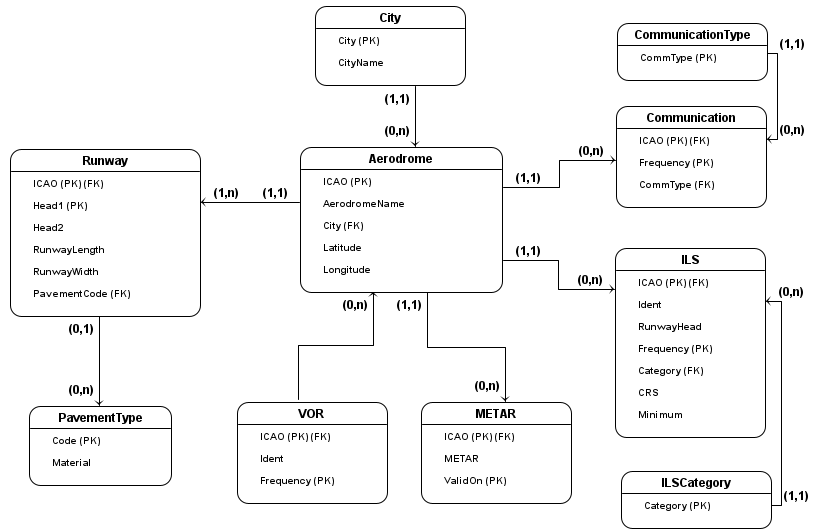
\includegraphics[width=400pt]{img/ERAero.png}
    \caption{Diagrama E/R}
    \label{fig:diagrama-er}
    \end{center}
\end{figure}

Note que as tabelas "CommunicationType", "ILSCategory" e "PavementType" poderiam ser substituídas
por colunas enum nas tabelas "Communication", "ILS" e "Runway", porém a manutenção seria difícil
\cite{table-enum},
pois teríamos que alterar a estrutura das tabelas (possivelmente tirando o sistema do ar) caso 
fosse necessário adicionar um tipo novo
de comunicação, por exemplo. Fazendo com uma tabela externa é necessário apenas adicionar uma nova
linha.

\section{Tabelas}

\begin{longtable}{|p{3cm}|p{6.6cm}|p{3cm}|}
    \caption{City} \\
    \hline
    \textbf{Nome} & \textbf{Descrição} & \textbf{Tipo} \\ \hline
    \endfirsthead
    \multicolumn{3}{c}%
    {{\tablename\ \thetable{} -- Continuação da página anterior}} \\
    \hline
    \textbf{Nome} & \textbf{Descrição} & \textbf{Tipo} \\ \hline
    \endhead
    \hline \multicolumn{3}{|r|}{{Continua na próxima página}} \\ \hline
    \endfoot
    \hline
    \endlastfoot
        City (PK)
        & Código do IBGE \cite{IBGE-cidade} da cidade
        & INTEGER
        \\ \hline
        CityName
        & Nome da cidade escrito em Português com a primeira letra maiúscula
        & VARCHAR (50)
        \\ \hline
\end{longtable}


\begin{longtable}{|p{3cm}|p{6.6cm}|p{3cm}|}
    \caption{Aerodrome} \\
    \hline
    \textbf{Nome}       & \textbf{Descrição} & \textbf{Tipo}  \\ \hline
    \endfirsthead
    \multicolumn{3}{c}%
    {{\tablename\ \thetable{} -- Continuação da página anterior}} \\
    \hline
    \textbf{Nome}       & \textbf{Descrição} & \textbf{Tipo}  \\ \hline
    \endhead
    \hline \multicolumn{3}{|r|}{{Continua na próxima página}} \\ \hline
    \endfoot
    \hline
    \endlastfoot
        ICAO (PK)
        & O código ICAO do aeródromo emitido pela Organização Internacional de Aviação Civil (ICAO).
        & VARCHAR(4)
        \\ \hline

        AerodromeName
        & O nome do aeródromo conforme definido pelo AISWEB, sistema nacional de informações aeronáuticas.
        & VARCHAR(50) 
        \\ \hline

        City (FK)
        & Chave estrangeira para o código da cidade
        & INTEGER
        \\ \hline

        Latitude 
        & A latitude do aeroporto em graus no formato de graus decimais (DD, Decimal Degrees). Três dígitos para 
        representar a parte inteira e seis dígitos para a fracionária.
        & DECIMAL(9, 6)
        \\ \hline
        
        Longitude 
        & A longitude do aeroporto, seguindo o mesmo formato da latitude. 
        & DECIMAL(9, 6)
        \\ \hline
\end{longtable}

\begin{longtable}{|p{3cm}|p{6.6cm}|p{3cm}|}
    \caption{METAR} \\
    \hline
    \textbf{Nome}       & \textbf{Descrição} & \textbf{Tipo}  \\ \hline
    \endfirsthead
    \multicolumn{3}{c}%
    {{\tablename\ \thetable{} -- Continuação da página anterior}} \\
    \hline
    \textbf{Nome}       & \textbf{Descrição} & \textbf{Tipo}  \\ \hline
    \endhead
    \hline \multicolumn{3}{|r|}{{Continua na próxima página}} \\ \hline
    \endfoot
    \hline
    \endlastfoot
        ICAO (PK) (FK)
        & Chave estrangeira para qual aeródromo este METAR se refere
        & VARCHAR(4)
        \\ \hline

        METAR
        & O METAR em si
        & VARCHAR(100)
        \\ \hline

        ValidOn (PK)
        & Timestamp com o momento que este metar é válido. É construído a
        partir do item do metar "ddhhmmZ" em que "dd" é o dia e "hhmm" é
        a hora zulu (UTC). O mês e ano são o mês e ano atuais do sistema.
        & DATETIME

        \\ \hline
\end{longtable}


\begin{longtable}{|p{3cm}|p{6.6cm}|p{3cm}|}
    \caption{PavementType} \\
    \hline
    \textbf{Nome}       & \textbf{Descrição}                                                                                          & \textbf{Tipo} \\ \hline
    \endfirsthead
    \multicolumn{3}{c}%
    {{\tablename\ \thetable{} -- Continuação da página anterior}} \\
    \hline
    \textbf{Nome}       & \textbf{Descrição}                                                                                          & \textbf{Tipo} \\ \hline
    \endhead
    \hline \multicolumn{3}{|r|}{{Continua na próxima página}} \\ \hline
    \endfoot
    \hline
    \endlastfoot

        Code (PK)
        & O código (em Inglês) do tipo de pavimento usado. É formado por três letras maiúsculas.
        & VARCHAR(3)
        \\ \hline

        Material 
        & O nome do pavimento em Português, com a primeira letra maiúscula.
        & VARCHAR(20)
        \\ \hline


\end{longtable}

\begin{verbatim}
Exemplo de siglas:

Code    Material
ASP     Asfalto
CON     Concreto
GVL     Brita
\end{verbatim}


É importante conhecer as características dos tipos de pistas de 
pouso e decolagem, pois seu comprimento determinará a quantidade de freio 
necessária para parar uma determinada aeronave.

Se a pista for muito curta, determinados modelos de avião não poderão pousar. 
A largura da pista determina a envergadura máxima que uma aeronave pode ter 
para operar nessa pista. Se uma pista for muito estreita, uma aeronave quadrimotora 
como o Boeing 747 pode sofrer ingestão de materiais, já que os dois motores mais 
externos ficarão para fora da área da pista, sobre o gramado.

\begin{longtable}{|p{3cm}|p{6.6cm}|p{3cm}|}
    \caption{Runway} \\
    \hline
    \textbf{Nome}       & \textbf{Descrição}                                                                                          & \textbf{Tipo} \\ \hline
    \endfirsthead
    \multicolumn{3}{c}%
    {{\tablename\ \thetable{} -- Continuação da página anterior}} \\
    \hline
    \textbf{Nome}       & \textbf{Descrição}                                                                                          & \textbf{Tipo} \\ \hline
    \endhead
    \hline \multicolumn{3}{|r|}{{Continua na próxima página}} \\ \hline
    \endfoot
    \hline
    \endlastfoot

        ICAO (FK e PK) 
        & O código ICAO do aeródromo ao qual a pista está associada, utilizado como chave estrangeira 
        fazendo a ligação com a tabela 'Aerodrome'.
        & VARCHAR(4)
        \\ \hline

        Head1 (PK) 
        & Número e possível letra que identifica uma das cabeceiras da pista. Um aeroporto nunca terá
        cabeceiras repetidas, então ICAO e Head1 formam uma chave primária mínima.
        & VARCHAR(3)
        \\ \hline

        Head2 (PK) 
        & O mesmo, mas para o outra cabeceira.
        & VARCHAR(3)
        \\ \hline

        RunwayLength
        & Comprimento da pista em metros.
        & INTEGER
        \\ \hline

        RunwayWidth
        & Largura da pista em metros.
        & INTEGER
        \\ \hline

        PavementCode (FK)
        & O tipo de pavimento da pista, referenciando a tabela 'PavementType'.
        & VARCHAR(3)
        \\ \hline

\end{longtable}

Para cabeceiras paralelas, ou seja, que apontam para a mesma direção, temos:

\subsection{Pista única}

A proa em que a pista aponta, com divisão por 10 arredondada. Por exemplo, em Fortaleza,
temos uma cabeceira com curso de 126 graus, dividindo por 10 temos 12,6, arredondando
temos o número 13 da cabeceira.

\subsection{Pista dupla}

Para duas pistas paralelas, usamos L para a cabeceira da esquerda e R para a da direita.
Por exemplo, no Santos Dumont, de costas para o Pão de Açúcar, temos as cabeceiras 02L 
(na esquerda) e 02R (na direita).

\subsection{Pista tripla}

Não temos aeroportos com três pistas paralelas no Brasil, mas são usadas as letras
L, C e R. C para a pista central.


\begin{longtable}{|p{3cm}|p{6.6cm}|p{3cm}|}
    \caption{CommunicationType} \\
    \hline
    \textbf{Nome}       & \textbf{Descrição}                                                                                          & \textbf{Tipo} \\ \hline
    \endfirsthead
    \multicolumn{3}{c}%
    {{\tablename\ \thetable{} -- Continuação da página anterior}} \\
    \hline
    \textbf{Nome}       & \textbf{Descrição}                                                                                          & \textbf{Tipo} \\ \hline
    \endhead
    \hline \multicolumn{3}{|r|}{{Continua na próxima página}} \\ \hline
    \endfoot
    \hline
    \endlastfoot

        CommType (PK)
        & O tipo de comunicação, podendo ser "Torre", "Solo", "ATIS", "Tráfego" ou "Operação".
        Mais adiante outros tipos podem ser adicionados.
        & VARCHAR(10)
        \\ \hline

\end{longtable}


\begin{longtable}{|p{3cm}|p{6.6cm}|p{3cm}|}
    \caption{Communication} \\
    \hline
    \textbf{Nome}       & \textbf{Descrição}                                                                                          & \textbf{Tipo} \\ \hline
    \endfirsthead
    \multicolumn{3}{c}%
    {{\tablename\ \thetable{} -- Continuação da página anterior}} \\
    \hline
    \textbf{Nome}       & \textbf{Descrição}                                                                                          & \textbf{Tipo} \\ \hline
    \endhead
    \hline \multicolumn{3}{|r|}{{Continua na próxima página}} \\ \hline
    \endfoot
    \hline
    \endlastfoot

        ICAO (PK e FK)
        & O código ICAO do aeródromo ao qual a frequência de comunicação está associada, utilizado 
        como chave estrangeira referenciando a tabela 'Aerodrome'.
        & VARCHAR(4)
        \\ \hline

        Frequency (PK)
        & A frequência em MHz multiplicada por 1000. Já que as frequências de comunicação possuem 
        três digitos decimais, multiplicamos por mil para armazenar em inteiro de ponto fixo. 
        ICAO e frequency formam chave primária e usar um DECIMAL para uma PK, não é muito eficiente. 
        Note que uma frequência, não necessariamente é única em todo o país, para distâncias longas, 
        onde não há risco de interferência, é possível haver frequências repetidas.
        & INTEGER
        \\ \hline

        CommType (FK)
        & O tipo de comunicação, chave estrangeira para 'CommunicationType'.
        & VARCHAR(20)
        \\ \hline

\end{longtable}


Esta tabela lista as diferentes categorias de Sistema de Pouso por Instrumentos
 (Instrument Landing System).

 \begin{longtable}{|p{3cm}|p{6.6cm}|p{3cm}|}
    \caption{ILSCategory} \\
    \hline
    \textbf{Nome}       & \textbf{Descrição}                                                                                          & \textbf{Tipo} \\ \hline
    \endfirsthead
    \multicolumn{3}{c}%
    {{\tablename\ \thetable{} -- Continuação da página anterior}} \\
    \hline
    \textbf{Nome}       & \textbf{Descrição}                                                                                          & \textbf{Tipo} \\ \hline
    \endhead
    \hline \multicolumn{3}{|r|}{{Continua na próxima página}} \\ \hline
    \endfoot
    \hline
    \endlastfoot

    Category (PK)
    & A categoria de ILS, sendo "CAT I", "CAT II", "CAT IIIA", "CAT IIIB" ou
    "CAT IIIC". Será explicado melhor em "Minimus" na tabela "ILS".
    & VARCHAR(10)
    \\ \hline

\end{longtable}

\begin{longtable}{|p{3cm}|p{6.6cm}|p{3cm}|}
    \caption{ILS} \\
    \hline
    \textbf{Nome}       & \textbf{Descrição}                                                                                          & \textbf{Tipo} \\ \hline
    \endfirsthead
    \multicolumn{3}{c}%
    {{\tablename\ \thetable{} -- Continuação da página anterior}} \\
    \hline
    \textbf{Nome}       & \textbf{Descrição}                                                                                          & \textbf{Tipo} \\ \hline
    \endhead
    \hline \multicolumn{3}{|r|}{{Continua na próxima página}} \\ \hline
    \endfoot
    \hline
    \endlastfoot

    ICAO (PK e FK)
    & O código ICAO do aeródromo ao qual o sistema de pouso está associado, utilizado 
    como chave estrangeira referenciando a tabela 'Aerodrome'.
    & VARCHAR(4)
    \\ \hline

    Frequency (PK)
    & A frequência de operação do ILS em MHz, multiplicado por 10. Fazemos isso para poder usar o tipo
    INTEGER, já que um DECIMAL como chave primária não seria eficiente, como já explicado na tabela de
    comunicação.
    & INTEGER
    \\ \hline

    Ident
    & Identificação de três letras maisculas única do ILS para aquele aeródromo.
    Aparece na carta aérea do procedimento ILS.
    & VARCHAR(3)
    \\ \hline

    RunwayHead
    & Para qual pista este ILS se refere.
    & VARCHAR(3)
    \\ \hline

    Category (FK)
    & A categoria do ILS, referenciando a tabela 'ILSCategory'.
    & VARCHAR(10)
    \\ \hline

    CRS
    & A referência do curso de aproximação do ILS. É a proa final que a aeronave deve 
    manter para o correto alinhamento nesta cabeceira.
    & INTEGER
    \\ \hline

    Minimum
    & A altura mínima de decisão em pés para operação do ILS. A partir desta altura, é
    desligado o piloto automático e o resto da aproximação é feita manualmente.
    Se a altitude da aeronave ficar abaixo deste valor e ainda não for possível 
    ter visual da pista é obrigatória a arremetida.
    
    Quando maior a categoria do ILS, maior a precisão do sistema, portanto a Minimus 
    será mais baixa. Uma "CAT IIIC" (pronuncia-se cat três charlie), possui Minimus zero, 
    portanto a aeronave pode pousar de forma totalmente automática.
    & INTEGER
    \\ \hline

\end{longtable}

Esta tabela registra os sistemas de navegação VOR/DME disponíveis em um aeródromo.
Não foi incluída uma tabela para as frequências de NDB porque este sistema
está caindo em desuso.

\begin{longtable}{|p{3cm}|p{6.6cm}|p{3cm}|}
    \caption{VOR} \\
    \hline
    \textbf{Nome}       & \textbf{Descrição}                                                                                          & \textbf{Tipo} \\ \hline
    \endfirsthead
    \multicolumn{3}{c}%
    {{\tablename\ \thetable{} -- Continuação da página anterior}} \\
    \hline
    \textbf{Nome}       & \textbf{Descrição}                                                                                          & \textbf{Tipo} \\ \hline
    \endhead
    \hline \multicolumn{3}{|r|}{{Continua na próxima página}} \\ \hline
    \endfoot
    \hline
    \endlastfoot

        ICAO (PK e FK)
        & O código ICAO do aeródromo ao qual o VOR/DME está associado, utilizado como 
        chave estrangeira referenciando a tabela 'Aerodrome'.
        & VARCHAR(4)
        \\ \hline

        Frequency (PK)
        & A frequência de operação do VOR/DME em MHz multiplicada por 10.
        & INTEGER
        \\ \hline

        Ident 
        & Identificação única do VOR/DME para aquele aeródromo. Forma chave primária
        junto com ICAO.
        & VARCHAR(3)
        \\ \hline

\end{longtable}

\section{Adicionado no Projeto II}

A tabela a seguir foi adicionada na segunda parte do Projeto. Ela serve para a autenticação
de usuário com senha e TOTP bem com gerenciar as permissões de cada usuário. 

\begin{longtable}{|p{3cm}|p{6.6cm}|p{3cm}|}
    \caption{Usuário} \\
    \hline
    \textbf{Nome} & \textbf{Descrição} & \textbf{Tipo} \\ \hline
    \endfirsthead
    \multicolumn{3}{c}%
    {{\tablename\ \thetable{} -- Continuação da página anterior}} \\
    \hline
    \textbf{Nome} & \textbf{Descrição} & \textbf{Tipo} \\ \hline
    \endhead
    \hline \multicolumn{3}{|r|}{{Continua na próxima página}} \\ \hline
    \endfoot
    \hline
    \endlastfoot

    Name (PK) & Nome do usuário. Usado no login. & VARCHAR(30) \\ \hline

    PasswordHash & Hash com salt da senha do usuário. A biblioteca bcrypt é usada
    para criação do hash e autenticação. & VARCHAR(60) \\ \hline

    TwoFactorKey & Chave privada para geração de código temporário de 6 dígitos
    comparado com o código digitado pelo usuário no momento do login. Pode ser nulo,
    caso não tenha sido cadastrada a autenticação de dois fatores, então essa
    verificação não é feita. & VARCHAR(32) \\ \hline

    CanEditAirportsList & Lista separada por vírgulas dos ICAOs dos aeroportos que
    este usuário tem permissão de alterar. Entenda "alterar" por criar, editar e
    apagar informações internas de um aeroporto: pistas, frequências de rádios e
    de navegação. & VARCHAR(32) \\ \hline

    IsSuper & Indica se o usuário pode criar e apagar aeroportos. Se verdadeiro,
    este usuário pode editar qualquer aeroporto, ignorando a lista CanEditAirportsList. 
    & Boolean \\ \hline
\end{longtable}
